\chapter{HASIL DAN PEMBAHASAN}

\section{Hasil Rancangan Sistem Identifikasi Kendaraan Pada Pemarkiran Dengan Pengenalan Citra Dan Pembacaan RFID}

\subsection{Hasil Perancangan Perangkat Keras}

\subsection{Raspberry Pi dan RFID MFRC522}
\begin{figure} [H]
    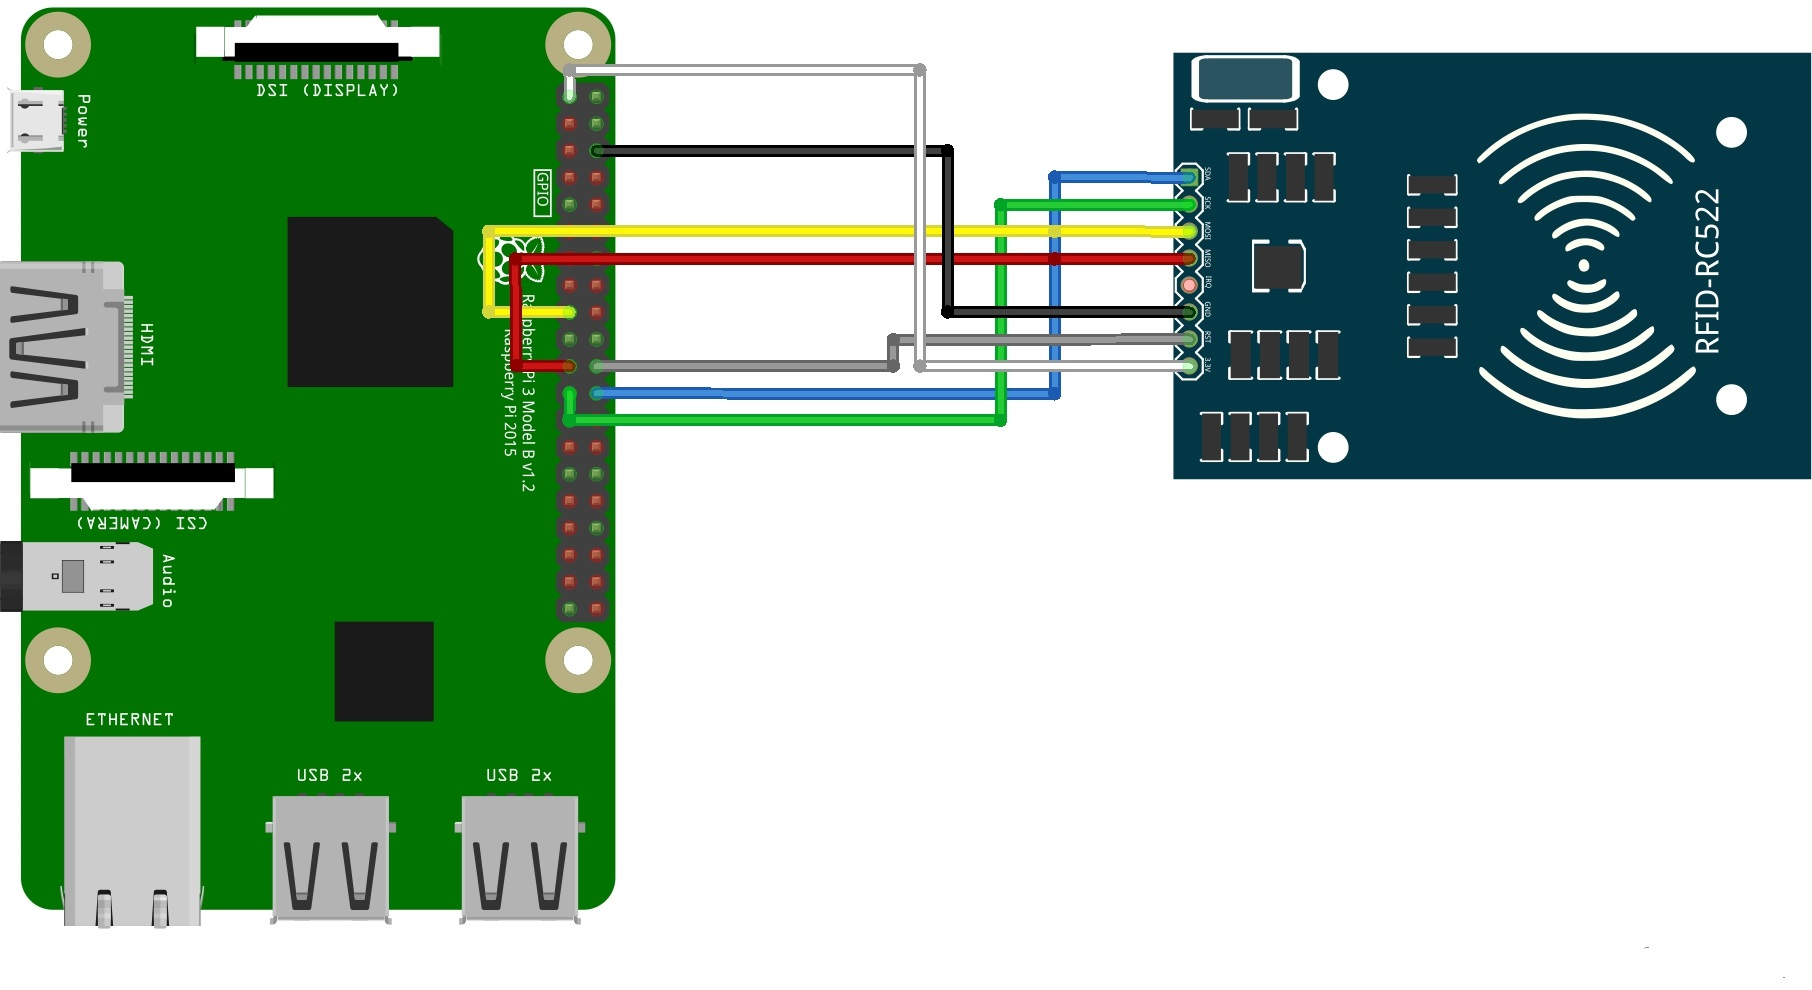
\includegraphics[width=0.85\textwidth, center]{images/skematik_rfid.jpg}
    \caption{Ragkaian Raspberry Pi dan RFID}
    \label{fig:skematikRfid}
\end{figure}

\begin{atable}
    \caption{Rangkaian pin RFID ke Raspberry Pi}
    \label{table:tableRfid}
    \csvreader[
        % column count = 11,
        tabular=cc,
        head to column names,
        before table=\rowcolors{2}{gray!15}{gray!30},
        table head= \rowcolor{gray!50!black} 
            \color{white} RFID & 
            \color{white} RASPBERRY PI 
            \\]
        {tables/tablerfid.csv}
        {
            RFID=\RFID, 
            RASPBERRYPI=\RASPBERRYPI}
        {
            \RFID & 
            \RASPBERRYPI}
\end{atable}

\subsection{Raspberry Pi dan HC-SR04}
\begin{figure} [H]
    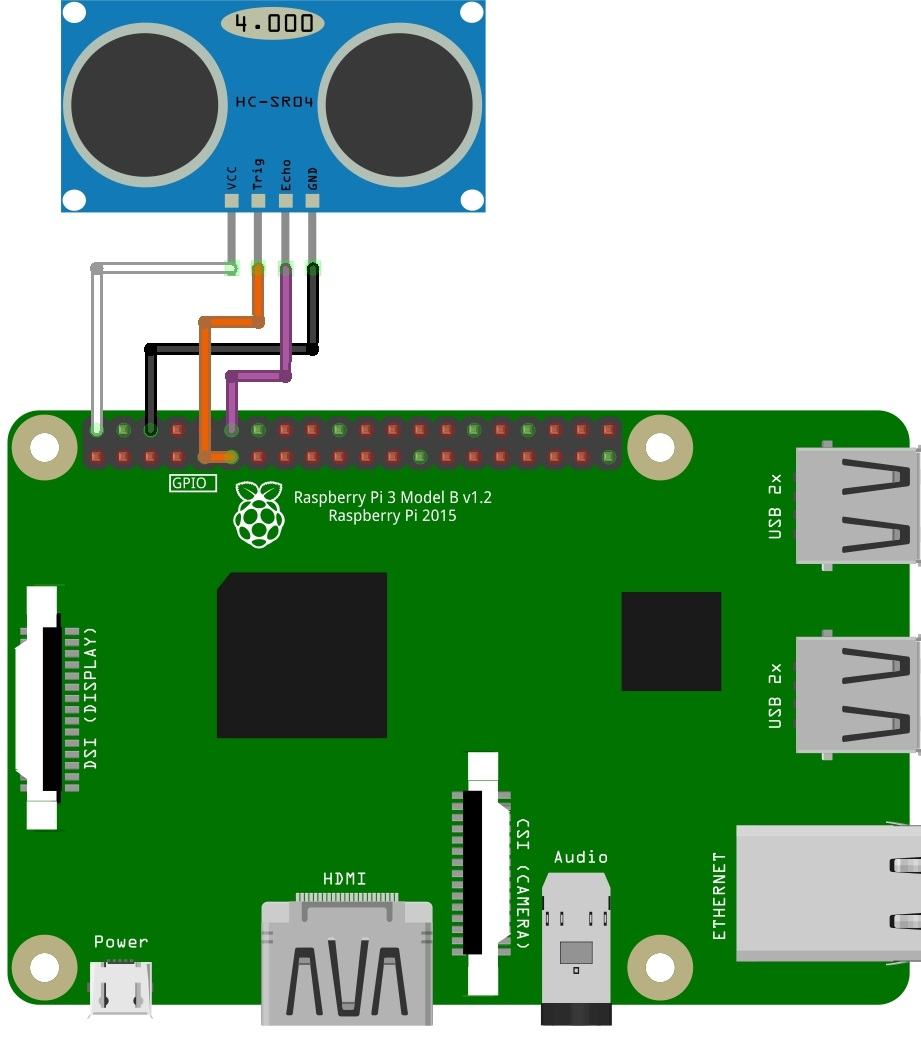
\includegraphics[height=7cm, width=0.5\textwidth, center]{images/skematik_ultra.jpg}
    \caption{Ragkaian Raspberry Pi dan Ultrasonik}
    \label{fig:skematikUltrasonik}
\end{figure}

\begin{atable}
    \caption{Rangkaian pin Ultrasonik ke Raspberry Pi}
    \label{table:tableUltrasonic}
    \csvreader[
        % column count = 11,
        tabular=cc,
        head to column names,
        before table=\rowcolors{2}{gray!15}{gray!30},
        table head= \rowcolor{gray!50!black} 
            \color{white} ULTRASONIK & 
            \color{white} RASPBERRY PI 
            \\]
        {tables/tableultrasonic.csv}
        {
            ULTRASONIC=\ULTRASONIC, 
            RASPBERRYPI=\RASPBERRYPI}
        {
            \ULTRASONIC & 
            \RASPBERRYPI}
\end{atable}

\subsection{Raspberry Pi dan SG90}
\begin{figure} [H]
    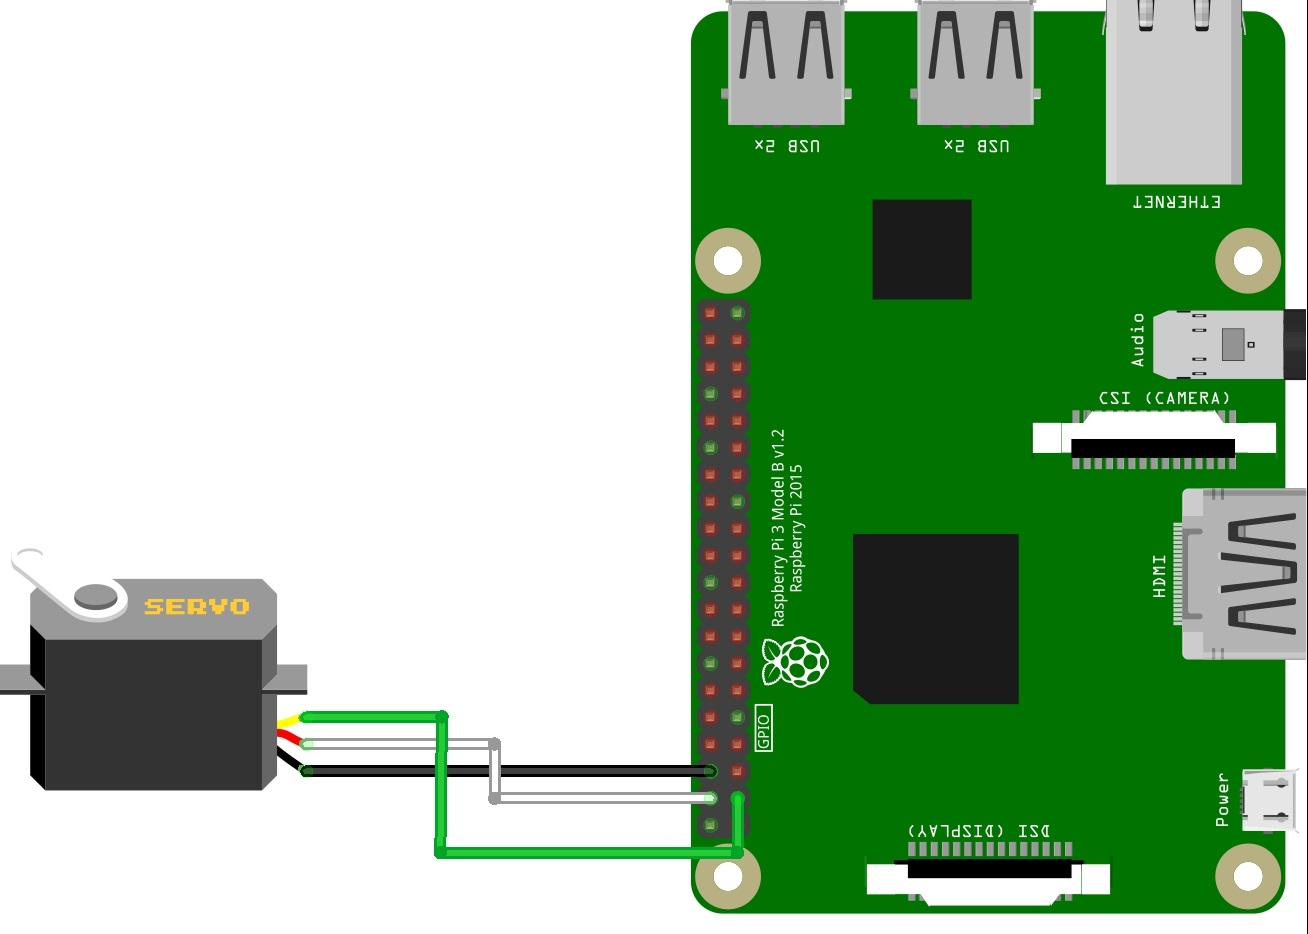
\includegraphics[height=7cm, width=0.6\textwidth, center]{images/skematik_servo.jpg}
    \caption{Ragkaian Raspberry Pi dan Servo}
    \label{fig:skematikServo}
\end{figure}

\begin{atable}
    \caption{Rangkaian pin Servo ke Raspberry Pi}
    \label{table:tableServo}
    \csvreader[
        % column count = 11,
        tabular=cc,
        head to column names,
        before table=\rowcolors{2}{gray!15}{gray!30},
        table head= \rowcolor{gray!50!black} 
            \color{white} SERVO & 
            \color{white} RASPBERRY PI 
            \\]
        {tables/tableservo.csv}
        {
            SERVO=\SERVO, 
            RASPBERRYPI=\RASPBERRYPI}
        {
            \SERVO & 
            \RASPBERRYPI}
\end{atable}

\subsection{Raspberry Pi dan Kamera Pi}

\subsection{Hasil Perancangan Perangkat Lunak}

\section{Hasil Rancangan Aplikasi Web}

\subsection{Activity Diagram}

\subsection{Struktur Database}

\subsection{Tampilan Website}